\documentclass{article}
\usepackage{amssymb}
\usepackage[utf8]{inputenc}
\usepackage{amsmath}
\usepackage{tikz}
\usepackage{color, colortbl}
\usepackage{amsmath}
\usepackage{tikz}
\usepackage[T1]{fontenc}
\usepackage{pgfplots}
\pgfplotsset{compat=1.17}

\begin{document}

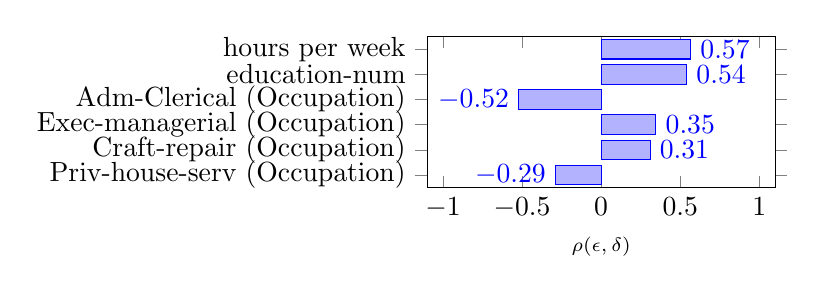
\begin{tikzpicture}
\begin{axis}[ 
xbar, xmin=-1.1,xmax=1.1,
xlabel={\scriptsize $\rho(\epsilon,\delta)$ },
symbolic y coords={%
    {Priv-house-serv (Occupation)},
    {Craft-repair (Occupation)},
    {Exec-managerial (Occupation)},
    {Adm-Clerical (Occupation)},
    {education-num},
    {hours per week}},
    bar width=0.25cm,
    height = 3.5cm,
    width = 6cm,
    xtick={-1,-0.5,0,0.5,1},
ytick=data,
nodes near coords, 
nodes near coords align={horizontal},
ytick=data,
]
\addplot coordinates {
    (-0.287845,{Priv-house-serv (Occupation)}) 
    (0.309775,{Craft-repair (Occupation)}) 
    (0.346542,{Exec-managerial  (Occupation)})
    (-0.521061,{Adm-Clerical (Occupation)})
    (0.541314,{education-num}) 
    (0.566165,{hours per week})};
\end{axis}
\end{tikzpicture}

\end{document}